%M2I Project proposal template
%Matthew E. Nelson
%Iowa State University
%8/15/2014
%Revision 1

\documentclass[10pt,foldmark,notumble]{leaflet}
\renewcommand*\foldmarkrule{.3mm}
\renewcommand*\foldmarklength{5mm}

%Packages we will be using
%\usepackage{amsmath}
\usepackage[T1]{fontenc}
\usepackage{textcomp}
\usepackage{float}
\usepackage{wrapfig}
\usepackage{mathptmx}
\usepackage[scaled=0.9]{helvet}
\makeatletter
\def\ptmTeX{T\kern-.1667em\lower.5ex\hbox{E}\kern-.075emX\@}
\DeclareRobustCommand{\ptmLaTeX}{L\kern-.3em
        {\setbox0\hbox{T}%
         %\vb@xt@ % :-)
         \vbox to\ht0{\hbox{%
                            \csname S@\f@size\endcsname
                            \fontsize\sf@size\z@
                            \math@fontsfalse\selectfont
                            A}%
                      \vss}%
        }%
        \kern-.12em
        \ptmTeX}
\makeatother
\let\TeX=\ptmTeX
\let\LaTeX=\ptmLaTeX
\usepackage{shortvrb}
\MakeShortVerb{\|}
\usepackage{url}
\usepackage{graphicx}
\usepackage[dvipsnames,usenames]{color}

%Define some colors used
\definecolor{LIGHTGRAY}{gray}{.9}
\definecolor{orange}{RGB}{255,127,0}
\definecolor{cardinal}{RGB}{206,17,38}
\definecolor{light-red}{RGB}{255,230,230}
\definecolor{gold}{RGB}{242,191,73}

\renewcommand{\descfont}{\normalfont}
\newcommand\Lpack[1]{\textsf{#1}}
\newcommand\Lclass[1]{\textsf{#1}}
\newcommand\Lopt[1]{\texttt{#1}}
\newcommand\Lprog[1]{\textit{#1}}

\newcommand*\defaultmarker{\textsuperscript\textasteriskcentered}


\title{\bf \ \\ Make to Innovate}

\author{%
\Large \bf \ \\ Iowa State University
}
\date{\bf Fall 2014 - Spring 2015}

\CutLine*{1}% Dotted line without scissors
\CutLine*{6}%  Dotted line without scissors

\AddToBackground{1}{
  \put(85,520){\includegraphics[scale=0.7]{images/M2I_logo_sm.png}}}


\AddToBackground*{2}{
  \put(\LenToUnit{.5\paperwidth},\LenToUnit{.5\paperheight}){%
    \makebox(0,0)[c]{%
      \resizebox{.9\paperwidth}{!}{\rotatebox{35.26}{%
        \textsf{\textbf{\textcolor{light-red}{M:2:I}}}}}}}}

\begin{document}
\maketitle
\section{What is M:2:I?} Make To Innovate (M:2:I) is an exciting new program in the Aerospace Engineering Department that engages students in hands-on projects to augment their understanding of engineering fundamentals.  

In a recent testimony to Congress, Regina Dugan, the DARPA Director, spoke of one of our Nations biggest challenges: the decline in our ability to make things.  Simply stated, "to innovate, we must be able to make".  We intend to re-energize our approach to design by introducing "Make to Innovate" or simply "M:2:I", in which students will learn how to design and operate a wide variety of projects in multi-disciplinary systems.  They will have the opportunity to design, build, and through testing they will be able to break things to learn from their failures.  We are also introducing students to some of the complexity of systems and the concept of design optimization, concepts they will carry forth throughout their career.

M:2:I currently has a number of projects that span a wide area of interests.  We literally have projects that span from underwater to space and everything in between.  
\begin{itemize}
\item Water based (underwater vehicles, boats)
\item Ground based (rovers)
\item Aero based (UASs, rockets, aircrafts)
\item Space based (High Altitude Balloons, Cubesat)
\end{itemize}

\section{About M:2:I}

\subsection{M:2:I History}
All sorts of interesting projects have spawned from M:2:I, but where did M:2:I come from? The group started in the Fall of 2011, but many of the projects in M:2:I have been around for five, ten, or even fifteen years or more. M:2:I was formed to give students hands on experience and consolidated two existing programs into one unified program.  This new program was then granted a new and much larger facility for the students to use.  M:2:I began with about 9 projects and 60 students.  Today M:2:I has close to 22 projects and well over 170 students involved and continues to grow.
\subsection{M:2:I Facilities}
The M:2:I Complex is a dedicated lab space for student projects.  These new facilities will be available for projects and will have controlled access to a wide-range of tools and electronics.  The lab is under the supervision of Matthew Nelson, the M:2:I Program Coordinator.  The lab is monitored by student technicians and lab monitors during the following hours:

\begin{center}
\vspace{0.2cm}
{\large \bf 0620 Lab}

\vspace{0.2cm}
{\bf Monday - Thursday}

12:00 pm -- 7:00 pm

\vspace{0.2cm}
{\bf Friday}

12:00 pm -- 5:00 pm

\vspace{0.2cm}
{\bf Saturday}

10:00 am -- 4:00 pm

These hours are subject to change, please see hours posted or check the website for additional information.
\end{center}

%\begin{wrapfigure}{R}{0.45\textwidth}
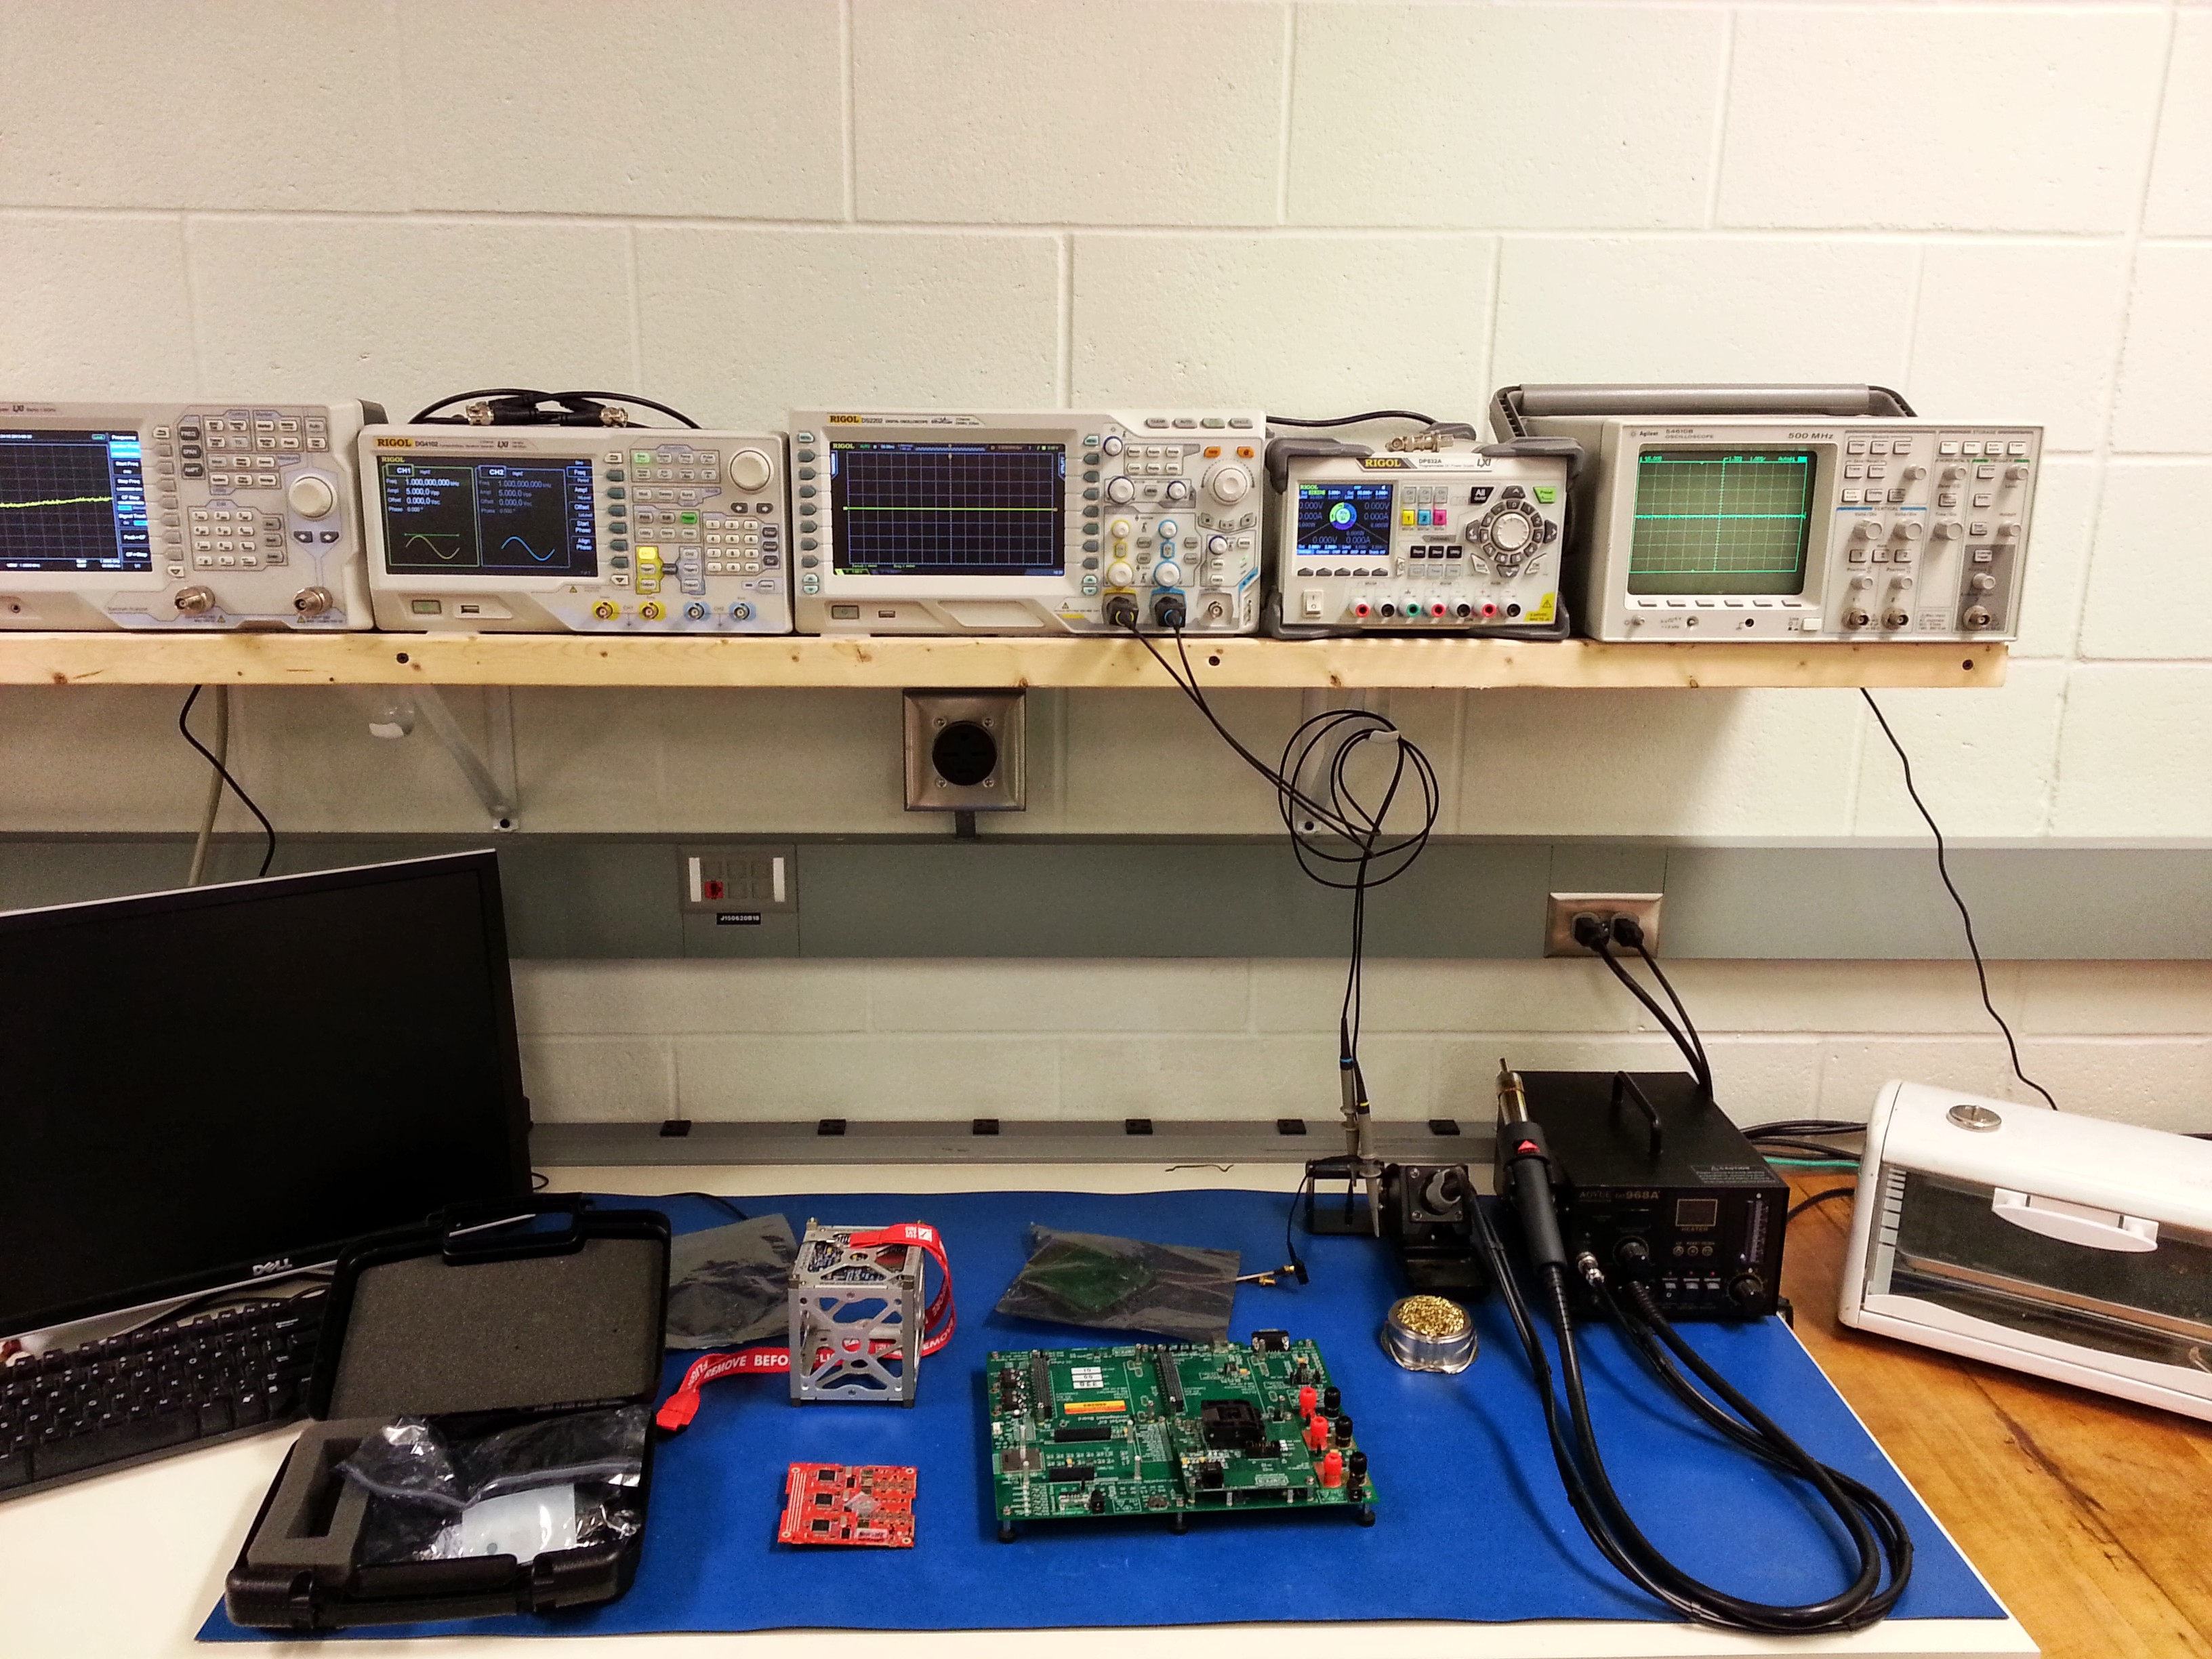
\includegraphics[scale=.068]{images/0620elab.jpg}
%\end{wrapfigure}
Additional times can be arranged through a request form in 0620.

The M:2:I Complex is located in 0620 Howe Hall and houses an assembly area, fabrication area, electronics lab, computer lab, Rapid Prototype Lab, project storage and a conference room.  In addition, we have access to 0618 for larger projects and 0638 for composites work.  M:2:I students can also get access to the workshop located in 1380 and are able to utilize additional 3D printers and two CNC machines through a job submission process.  1380 also has a table saw and other wood working equipment.

\section{Why Should I Join?}

There are a number of reasons to join M:2:I.  Here are just a few reasons to join.

\subsection{Future Employers}
M:2:I works with several companies in a large variety of industries.  These companies support M:2:I through both financial contributions and by working directly with the students.  We currently have Rockwell Collins, Boeing and others that support M:2:I.  This allows students to start networking with potential employers early in their academic careers.  We have also had several employers tell us that activities like M:2:I is what they like to see on a resume, so being involved can help your resume when you graduate from Iowa State University.

\subsection{A Great Community}
M:2:I is successful because of our students.  We have a great community and students involved in M:2:I often work together on homework and helping each other outside of their M:2:I project.  M:2:I offers a great way for you to network with your fellow students.

\subsection{Learn Valuable Skills}
While working on your M:2:I project will learn valuable skills that can't be taught in a normal classroom environment.  Students will gain a better appreciation for how ideas get transformed to actual hardware and a final product.  In addition, many students will learn how to use a variety of tools and equipment that they may not otherwise have access to.  We encourage students to sign up for projects that under M:2:I and get course credit for doing so (AerE 290 and AerE 490).  These projects will be interesting to our students and include projects drawn directly from industry, from ideas developed within the department and from external competitions.  All students within the Department are encouraged to get involved at any time during their educational program.  We also encourage students outside of our department to participate in multidisciplinary teams.

\section{How Do I Join?}

\begin{enumerate}
\item Speak with your adviser
\item Contact Matthew Nelson (mnelson@iastate.edu)
\item Find a project to get involved in (or submit your own)
\item Sign up for AerE 290C MN or AerE 490E MN.
\end{enumerate}

That's it!  It's that simple!

\section{Contact Information}

\begin{center}
Contact Information:

Matthew E. Nelson

M:2:I Program Coordinator

mnelson@iastate.edu
\ \\ \ \\
James Benson

Student Projects and Lab Coordinator

jdbenson@iastate.edu
\end{center}

Find us on the web:

Website-\url{http://www.aere.iastate.edu/m2i}

Facebook-\url{http://www.facebook.com/make2innovate}

Google+\url{http://plus.google.com/113581233284865216858}

Twitter- \url{http://www.twitter.com/make2innovate}

%\begin{wrapfigure}{R}{0.45\textwidth}
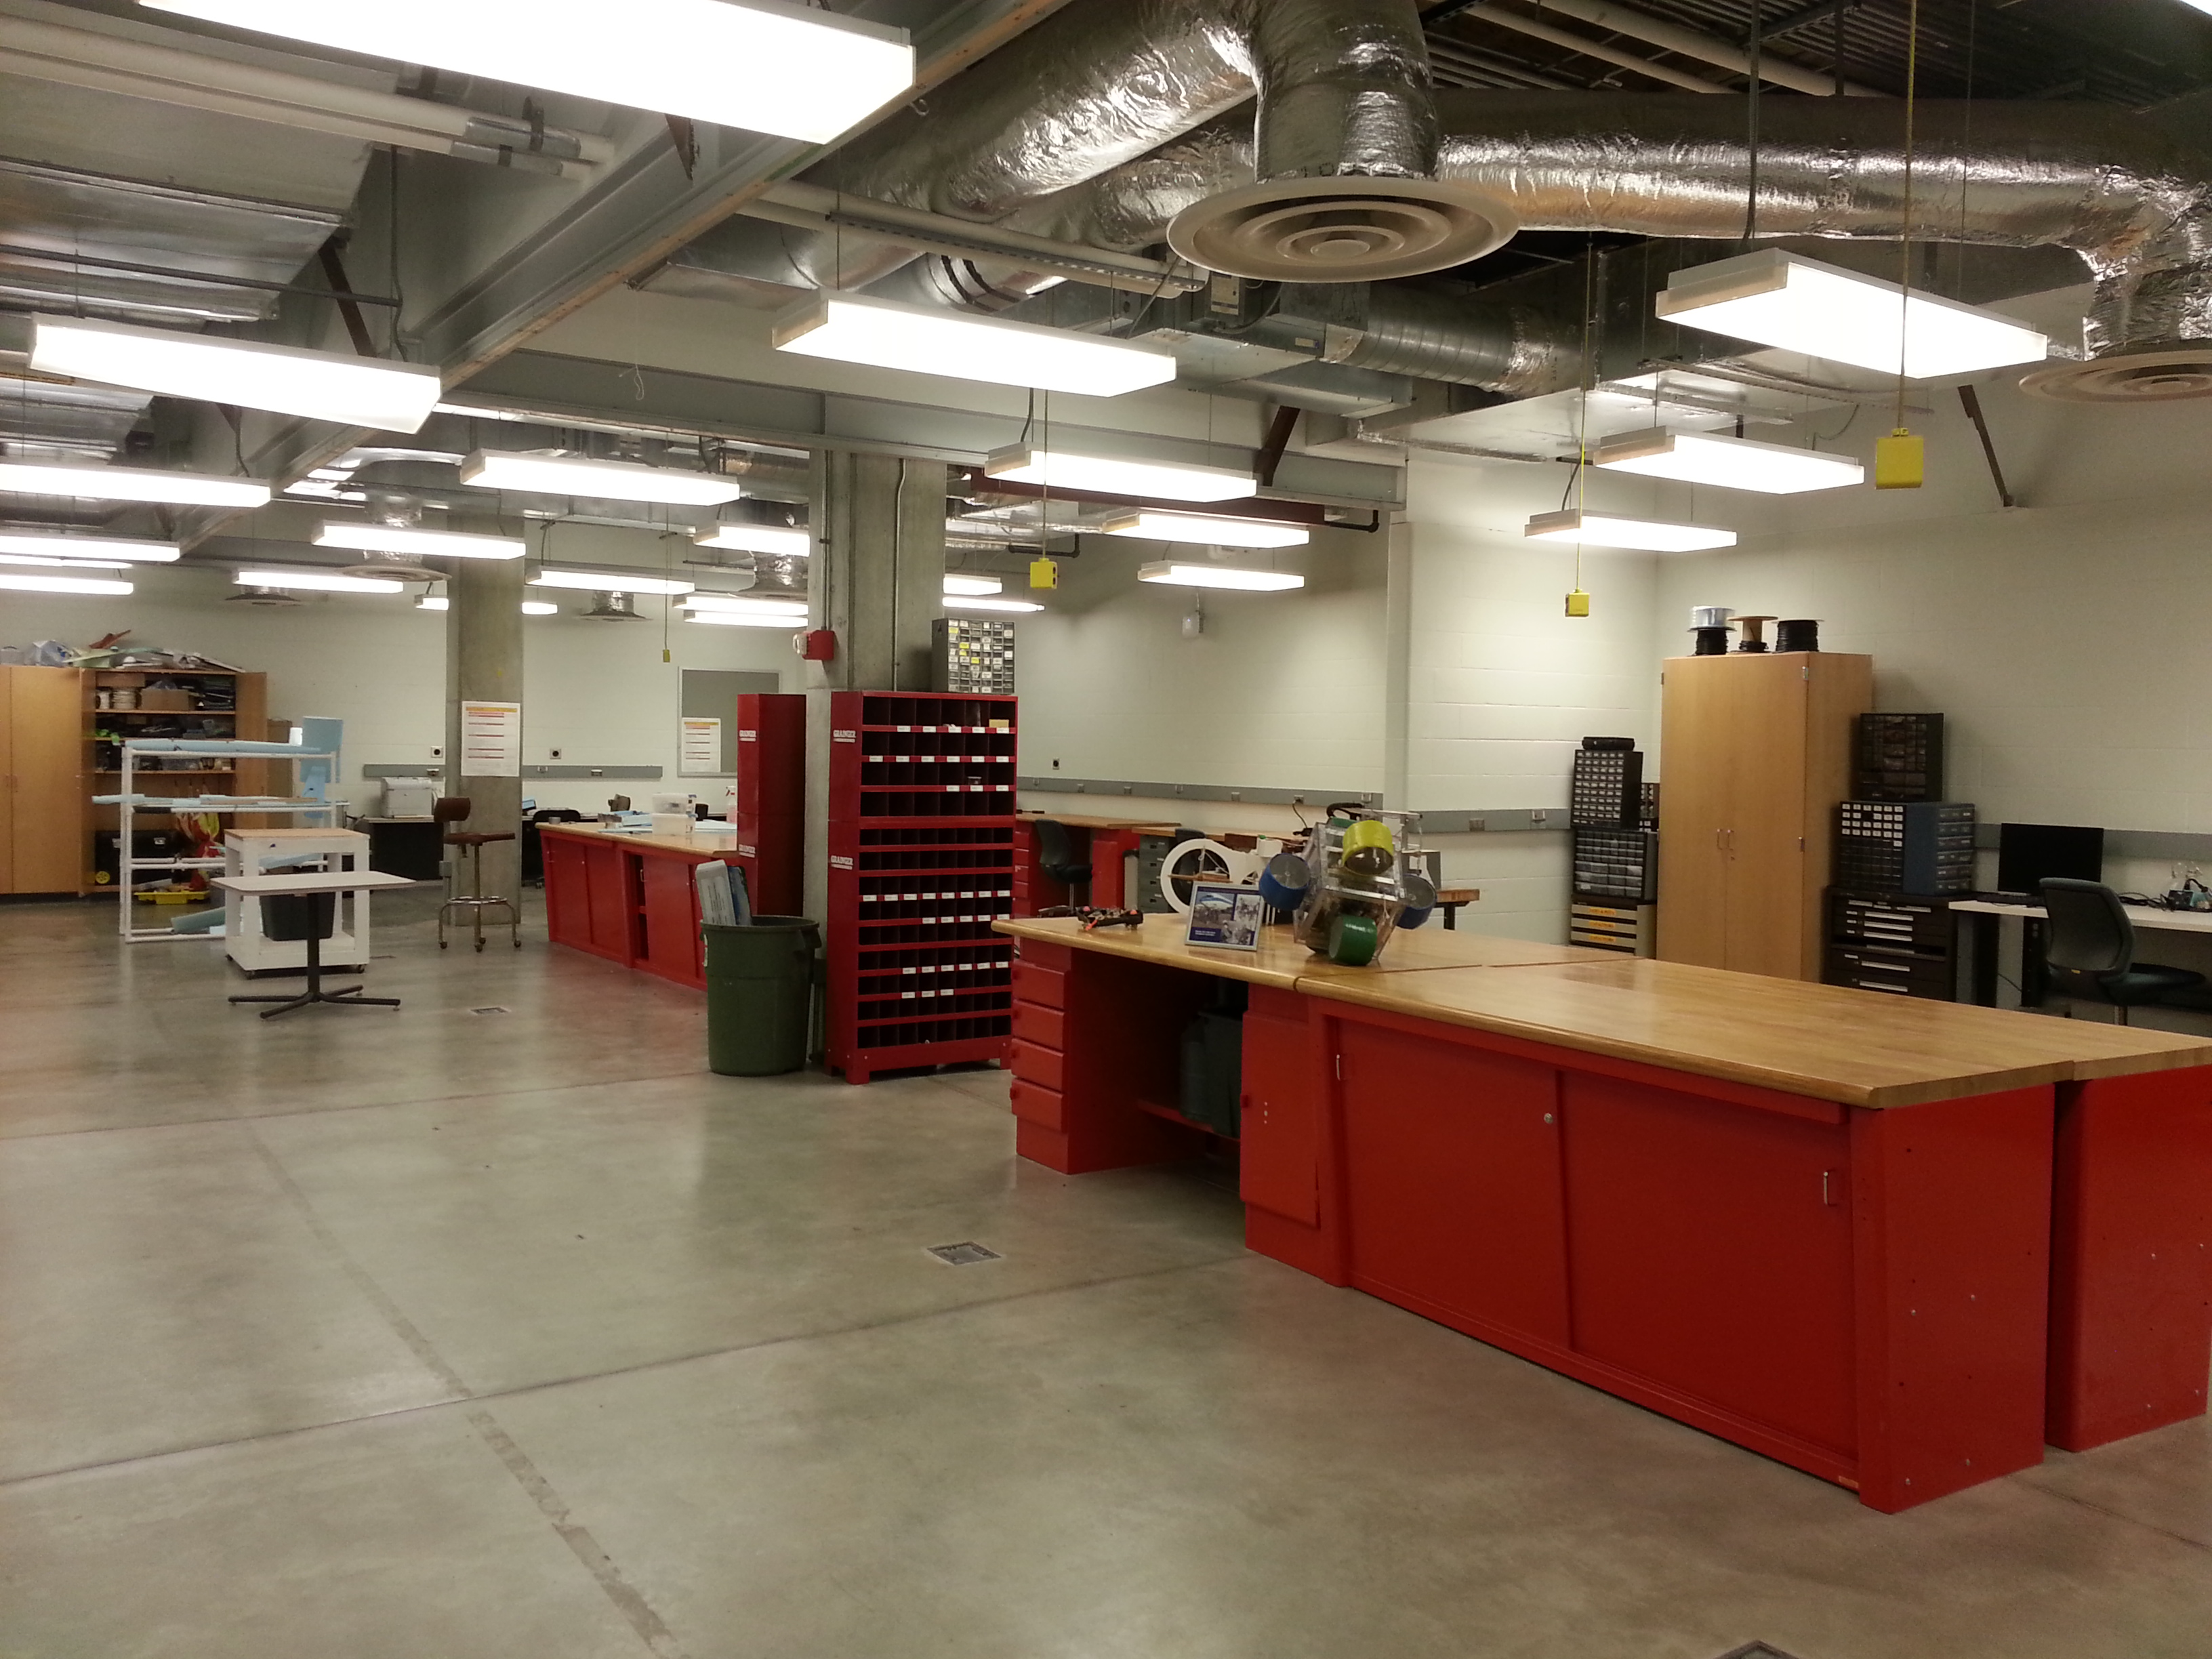
\includegraphics[scale=.07]{images/0620_lab.jpg}
%\end{wrapfigure}
\section{Projects}
An updated list of projects can be found on our website, http://www.aere.iastate.edu/m2i/team-projects/

\section{FAQ}
\textbf{How many project teams are there?} \ \\
\textit{Between fifteen and twenty-five. The number changes every year, depending on a number of factors.}\ \\ 
\textbf{What are the sizes of the groups?}\ \\
\textit{Four to fifteen members. The group sizes depend on the number of people needed for the project and how many want to be involved.}\ \\
\textbf{Where does the funding come from?}\ \\
\textit{M:2:I is funded by the Aerospace Engineering department and through private and corporate sponsors.}\ \\ 
\textbf{What are the requirements to join?}\ \\
\textit{Any ISU student can join.  Students must also enroll in the AerE 290 or 490 course as well.  Students do not have to be in the Aerospace Engineering department or even the college of engineering, all students are encouraged to get involved.}\ \\
\textbf{Is M:2:I a class?}\ \\
\textit{Yes! It is a 1-3 credit lab class. (AER E majors can earn up to 6 technical elective credits).}\ \\
\textbf{What is the time commitment?}\ \\
\textit{Depending on the work load of your project, anywhere from 3-15/hours a week.}\ \\
\textbf{Are there leadership positions?}\ \\
\textit{There is the opportunity to start and lead your own project or there are opportunities to work your way up through another group by being actively involved.}\ \\ 
\textbf{What are the meeting times?}\ \\
\textit{It varies on an individual group basis. Check the M:2:I website which has a calendar of all meetings and other M:2:I events.}\ \\
\textbf{Can I make my own project?}\ \\
\textit{Yes! You will need to submit a project proposal and visit with Matthew Nelson.  Information can be found on the M:2:I website.}\ \\
\textbf{What do you do when a project is finished?}\ \\
\textit{Most projects are ongoing projects and continue from semester to semester.  If you are involved in a project that does end, we have lots of other projects for you to get involved in.  We want to see students involved in M:2:I the entire time they are with us at ISU.}\ \\
\textbf{How does M:2:I help me?}\ \\
\textit{Students gain valuable hands on experience outside of the classroom.  In addition, since M:2:I partners with corporations like Boeing and Rockwell, students can also gain connections to these companies.}\ \\

\end{document}